\documentclass[journal,12pt,twocolumn]{IEEEtran}
\usepackage{setspace}
\usepackage{gensymb}
\singlespacing
\usepackage[cmex10]{amsmath}
\usepackage{amsthm}
\usepackage{mathrsfs}
\usepackage{txfonts}
\usepackage{stfloats}
\usepackage{bm}
\usepackage{cite}
\usepackage{cases}
\usepackage{subfig}
\usepackage{longtable}
\usepackage{multirow}
\usepackage{enumitem}
\usepackage{mathtools}
\usepackage{tikz}
\usepackage{circuitikz}
\usepackage{verbatim}
\usepackage[breaklinks=true]{hyperref}
\usepackage{tkz-euclide} % loads  TikZ and tkz-base
\usepackage{listings}
\usepackage{color}    
\usepackage{array}    
\usepackage{longtable}
\usepackage{calc}     
\usepackage{multirow} 
\usepackage{hhline}   
\usepackage{ifthen}   
\usepackage{lscape}     
\usepackage{chngcntr}
\DeclareMathOperator*{\Res}{Res}
\renewcommand\thesection{\arabic{section}}
\renewcommand\thesubsection{\thesection.\arabic{subsection}}
\renewcommand\thesubsubsection{\thesubsection.\arabic{subsubsection}}

\renewcommand\thesectiondis{\arabic{section}}
\renewcommand\thesubsectiondis{\thesectiondis.\arabic{subsection}}
\renewcommand\thesubsubsectiondis{\thesubsectiondis.\arabic{subsubsection}}
\renewcommand\thetable{\arabic{table}}
% correct bad hyphenation here
\hyphenation{op-tical net-works semi-conduc-tor}
\def\inputGnumericTable{}                                 %%

\lstset{
%language=C,
frame=single, 
breaklines=true,
columns=fullflexible,
literate=
{-}{$\rightarrow{}$}{1},
}
%\lstset{
%language=tex,
%frame=single, 
%breaklines=true
%}

\DeclareMathOperator*{\argmax}{arg\,max}
\DeclareMathOperator*{\argmin}{arg\,min}
\begin{document}
\newtheorem{theorem}{Theorem}[section]
\newtheorem{problem}{Problem}
\newtheorem{proposition}{Proposition}[section]
\newtheorem{lemma}{Lemma}[section]
\newtheorem{corollary}[theorem]{Corollary}
\newtheorem{example}{Example}[section]
\newtheorem{definition}[problem]{Definition}
\newcommand{\BEQA}{\begin{eqnarray}}
\newcommand{\EEQA}{\end{eqnarray}}
\newcommand{\define}{\stackrel{\triangle}{=}}
\bibliographystyle{IEEEtran}
\providecommand{\mbf}{\mathbf}
\providecommand{\pr}[1]{\ensuremath{\Pr\left(#1\right)}}
\providecommand{\qfunc}[1]{\ensuremath{Q\left(#1\right)}}
\providecommand{\sbrak}[1]{\ensuremath{{}\left[#1\right]}}
\providecommand{\lsbrak}[1]{\ensuremath{{}\left[#1\right.}}
\providecommand{\rsbrak}[1]{\ensuremath{{}\left.#1\right]}}
\providecommand{\brak}[1]{\ensuremath{\left(#1\right)}}
\providecommand{\lbrak}[1]{\ensuremath{\left(#1\right.}}
\providecommand{\rbrak}[1]{\ensuremath{\left.#1\right)}}
\providecommand{\cbrak}[1]{\ensuremath{\left\{#1\right\}}}
\providecommand{\lcbrak}[1]{\ensuremath{\left\{#1\right.}}
\providecommand{\rcbrak}[1]{\ensuremath{\left.#1\right\}}}
\providecommand{\floor}[1]{\ensuremath{\lfloor #1 \rfloor}}
\providecommand{\lfloor}[1]{\ensuremath{\lfloor #1 \right.}}
\providecommand{\rfloor}[1]{\ensuremath{\left.#1 \rfloor}}
\theoremstyle{remark}
\newtheorem{rem}{Remark}
\newcommand{\sgn}{\mathop{\mathrm{sgn}}}
\newcommand{\re}{\mathop{\mathrm{Re}}}
\providecommand{\abs}[1]{\left\vert#1\right\vert}
\providecommand{\res}[1]{\Res\displaylimits_{#1}} 
\providecommand{\norm}[1]{\left\lVert#1\right\rVert}
\providecommand{\mtx}[1]{\mathbf{#1}}
\providecommand{\mean}[1]{E\left[ #1 \right]}   
\providecommand{\fourier}{\overset{\mathcal{F}}{ \rightleftharpoons}}
\providecommand{\system}[1]{\overset{\mathcal{#1}}{ \longleftrightarrow}}
\newcommand{\solution}{\noindent \textbf{Solution: }}
\newcommand{\cosec}{\,\text{cosec}\,}
\providecommand{\dec}[2]{\ensuremath{\overset{#1}{\underset{#2}{\gtrless}}}}
\newcommand{\myvec}[1]{\ensuremath{\begin{pmatrix}#1\end{pmatrix}}}
\newcommand{\mydet}[1]{\ensuremath{\begin{vmatrix}#1\end{vmatrix}}}
\renewcommand{\vec}[1]{\boldsymbol{\mathbf{#1}}}
\def\putbox#1#2#3{\makebox[0in][l]{\makebox[#1][l]{}\raisebox{\baselineskip}[0in][0in]{\raisebox{#2}[0in][0in]{#3}}}}
     \def\rightbox#1{\makebox[0in][r]{#1}}
     \def\centbox#1{\makebox[0in]{#1}}
     \def\topbox#1{\raisebox{-\baselineskip}[0in][0in]{#1}}
     \def\midbox#1{\raisebox{-0.5\baselineskip}[0in][0in]{#1}}

\vspace{3cm}
\title{Advanced DSP (EE5900)\\Homework Assignment 2}
\author{Gautam Singh\\CS21BTECH11018}
\maketitle
\bigskip

\begin{enumerate}[label=\theenumi.]
    \item Given impulse response of digital filter is
        \begin{equation}
            h\brak{n} = A\cos\brak{\omega_0n+\phi}u\brak{n}.
            \label{eq:h-n-1}
        \end{equation}
        The difference equation of the digital filter is
        \begin{equation}
            y\brak{n} = x\brak{n} + a_1y\brak{n-1} + b_1y\brak{n-2}.
            \label{eq:filt-1}
        \end{equation}
        Taking the \(Z\)-transform on both sides of \eqref{eq:filt-1},
        \begin{align}
            Y\brak{z} &= X\brak{z} + a_1z^{-1}Y\brak{z} + b_1z^{-2}Y\brak{z}.
        \end{align}
        Therefore,
        \begin{align}
            H\brak{z} &= \frac{Y\brak{z}}{X\brak{z}} = \frac{1}{1 - \brak{a_1z^{-1} + b_1z^{-2}}}.
            \label{eq:H-z-filt-1}
        \end{align}
        \begin{enumerate}
            \item Taking the \(Z\)-transform of \eqref{eq:h-n-1},
                \begin{equation}
                    H\brak{z} = \sum_{k=0}^{\infty}A\cos\brak{\omega_0k+\phi}z^{-k}.
                    \label{eq:H-z-1}
                \end{equation}
                Expanding \eqref{eq:H-z-filt-1},
                \begin{align}
                    H\brak{z} &= \sum_{k=0}^{\infty}\brak{a_1z^{-1}+b_1z^{-2}}^k \\
                    &= 1 + a_1z^{-1} + \brak{a_1^2+b_1}z^{-2} \nonumber \\
                    &+\brak{a_1^3+2a_1b_1}z^{-3} + \ldots.
                    \label{eq:H-z-direct}
                \end{align}
                Equating the coefficients of \eqref{eq:H-z-1} and
                \eqref{eq:H-z-direct}, we get
                \begin{align}
                    A\cos\phi &= 1 \label{eq:z0} \\
                    A\cos\brak{\frac{\pi}{4}+\phi} &= a_1 \label{eq:z1} \\
                    A\cos\brak{\frac{\pi}{2}+\phi} &= a_1^2 + b_1 \label{eq:z2} \\
                    A\cos\brak{\frac{3\pi}{4}+\phi} &= a_1^3 + 2a_1b_1. \label{eq:z3}
                \end{align}
                Using \eqref{eq:z0} in \eqref{eq:z1},
                \begin{align}
                    A\brak{\cos\phi - \sin\phi} &= \sqrt{2}a_1 \\
                    \implies A\sin\phi &= 1 - \sqrt{2}a_1.
                    \label{eq:A-sin-phi}
                \end{align}
                Using \eqref{eq:A-sin-phi} in \eqref{eq:z2},
                \begin{align}
                    a_1^2 - \sqrt{2}a_1 + b_1 + 1 = 0 \\
                    \implies b_1 = -a_1^2 + \sqrt{2}a_1 - 1.
                    \label{eq:b1-a1}
                \end{align}
                Using \eqref{eq:z0} and \eqref{eq:A-sin-phi} in \eqref{eq:z3},
                \begin{align}
                    a_1^3 + 2a_1b_1 + \frac{2 - \sqrt{2}a_1}{\sqrt{2}} &= 0 \\
                    \implies a_1^3 + 2a_1b_1 + \sqrt{2} - a_1 = 0.
                    \label{eq:a1-b1}
                \end{align}
                Using \eqref{eq:b1-a1} in \eqref{eq:a1-b1} and simplifying,
                \begin{align}
                    a_1^3 - 2\sqrt{2}a_1^2 + 3a_1 - \sqrt{2} &= 0 \\
                    \brak{a_1-\sqrt{2}}\brak{a_1^2-\sqrt{2}a_1+1} &= 0 \\
                    \brak{a_1-\sqrt{2}}\brak{\brak{a_1-\frac{1}{\sqrt{2}}}^2+\frac{1}{2}} &= 0 \\
                    \implies a_1 &= \sqrt{2}. \label{eq:sol-a1}
                \end{align}
                Substituting in \eqref{eq:b1-a1}, \(b_1 = -1\).

                \item We see that \(h\brak{1}\) in the unquantized digital
                filter is \(a_1 = \sqrt{2}\). However, after quantization,
                using \eqref{eq:z0} to \eqref{eq:z2},
                \begin{align}
                    h\brak{0} &= A\cos\phi = 1 \label{eq:qz0} \\
                    h\brak{1} &= A\cos\brak{\omega+\phi} = 1.375 \label{eq:qz1} \\
                    h\brak{2} &= A\cos\brak{2\omega+\phi} = 1, \label{eq:qz2}
                \end{align}
                where the right hand side of \eqref{eq:qz1} follows
                because \(\sqrt{2} = \brak{1.011\ldots}_2\). Using \eqref{eq:qz0}
                in \eqref{eq:qz2},
                \begin{align}
                    \cos2\omega - A\sin\phi\sin2\omega &= 1 \\
                    2\sin^2\omega + A\sin\phi\brak{2\sin\omega\cos\omega} &= 0 \\
                    \sin\omega\brak{A\sin\phi\cos\omega+\sin\omega} &= 0.
                    \label{eq:omega-q}
                \end{align}
                In \eqref{eq:omega-q}, if \(\sin\omega = 0\) or \(\omega =
                n\pi\), \eqref{eq:qz0} and \eqref{eq:qz1} contradict each other.
                Thus, we must have
                \begin{equation}
                    \tan\omega = -A\sin\phi.
                    \label{eq:omega-phi}
                \end{equation}
                Substituting \eqref{eq:omega-phi} in \eqref{eq:qz1},
                \begin{align}
                    \cos\omega + \tan\omega\sin\omega &= 1.375 \\
                    \implies \frac{1}{\cos\omega} &= \frac{11}{8} \\
                    \implies \cos\omega &= \frac{8}{11}.
                \end{align}
                Thus, on quantization, \(\omega =
                \cos^{-1}\brak{\frac{8}{11}}\).
        \end{enumerate}

    \item Given analog frequecy response,
    \begin{equation}
        H_a\brak{j\Omega} =
        \begin{cases}
            j\Omega{}e^{-j\Omega\tau} & \abs{\Omega} \le \Omega_c \\
            0 & \text{otherwise}
        \end{cases}.
        \label{eq:analog-resp}
    \end{equation}
    \begin{enumerate}
        \item Setting \(\Omega = \frac{\omega}{T}\), the frequency response
        of the digital filter obtained is
        \begin{equation}
            H_d\brak{e^{j\omega}} = 
            \begin{cases}
                j\frac{\omega}{T}e^{-j\frac{\omega}{T}\tau} & \abs{\omega} \le \Omega_cT \\
                0 & \text{otherwise}
            \end{cases}.
            \label{eq:digital-resp}
        \end{equation}

        \item From \eqref{eq:digital-resp}, setting \(\tau = 0\),
        \begin{equation}
            \hat{H_d}\brak{e^{j\omega}} = j\frac{\omega}{T}
            \label{eq:digital-resp-zero}
        \end{equation}
        Note that
        \begin{align}
            \hat{h_d}\brak{n-n_{\tau}} &\system{F} e^{-j\omega{}n_{\tau}}\hat{H_d}\brak{e^{j\omega}} \\
            &= j\frac{\omega}{T}e^{-j\omega{}n_{\tau}} =  j\frac{\omega}{T}e^{-j\omega\frac{\tau}{T}}.
            \label{eq:n-tau}
        \end{align}
        From \eqref{eq:n-tau}, since \(n_{\tau} \in \mathbb{Z}\), we see 
        that
        \begin{equation}
            \tau = kT,\ n_{\tau} = k\ \forall\ k \in \mathbb{Z}.
            \label{eq:sol-set}
        \end{equation}
    \end{enumerate}

    \item From \autoref{fig:lpf-init},
    \begin{figure}[!ht]
        \centering
        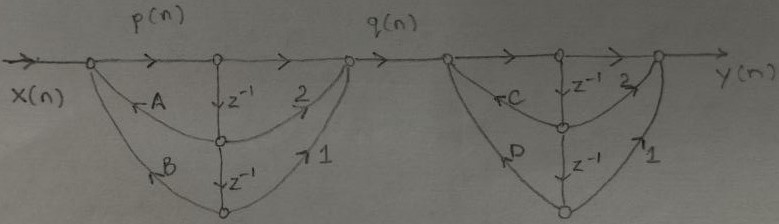
\includegraphics[width=\columnwidth]{figs/lpf-init.jpg}
        \caption{Lowpass Digital Filter.}
        \label{fig:lpf-init}
    \end{figure}
    \begin{align}
        p\brak{n} &= x\brak{n} + Ap\brak{n-1} + Bp\brak{n-2}, \label{eq:block-1} \\
        q\brak{n} &= p\brak{n} + 2p\brak{n-1} + p\brak{n-2}. \label{eq:block-2}
    \end{align}
    Taking the \(Z\)-transform on both sides of \eqref{eq:block-1} and
    \eqref{eq:block-2},
    \begin{align}
        P\brak{z}\brak{1-Az^{-1}-Bz^{-2}} = X\brak{z}, \label{eq:zblock-1} \\
        Q\brak{z} = P\brak{z}\brak{1+2z^{-1}+z^{-2}}. \label{eq:zblock-2}
    \end{align}
    From \eqref{eq:zblock-1} and \eqref{eq:zblock-2},
    \begin{equation}
        \frac{Q\brak{z}}{X\brak{z}} = \frac{\brak{1+z^{-1}}^2}{1-Az^{-1}-Bz^{-2}}
        \label{eq:trans-func-block}
    \end{equation}
    Since two similar blocks are cascaded, we see that the lowpass filter has
    transfer function
    \begin{align}
        H_{LP}\brak{z} &= \frac{Y\brak{z}}{X\brak{z}} \\
        &= \frac{\brak{1+z^{-1}}^4}{\brak{1-Az^{-1}-Bz^{-2}}\brak{1-Cz^{-1}-Dz^{-2}}}.
        \label{eq:trans-func-tot}
    \end{align}
    We apply the lowpass to highpass transform to \eqref{eq:trans-func-tot}. The
    given cutoff frequency of the lowpass filter is \(\omega_L = \frac{\pi}{2}\)
    and the required cutoff frequency of the highpass filter is \(\omega_H =
    \frac{\pi}{2}\). Thus,
    \begin{equation}
        \alpha = -\frac{\cos\brak{\frac{\omega_L+\omega_H}{2}}}{\cos\brak{\frac{\omega_L-\omega_H}{2}}} = 0
        \label{eq:alpha}
    \end{equation}
    and we must use the transformation
    \begin{equation}
        z^{-1} \rightarrow -\frac{z^{-1}+\alpha}{1+\alpha{}z^{-1}} = -z^{-1}.
        \label{eq:low-high-transform}
    \end{equation}
    Using \eqref{eq:low-high-transform} in \eqref{eq:trans-func-tot}, the 
    required highpass transfer function is
    \begin{align}
        &H_{HP}\brak{z} = \frac{\brak{1-z^{-1}}^4}{\brak{1+Az^{-1}-Bz^{-2}}\brak{1+Cz^{-1}-Dz^{-2}}} \\
        &= \frac{1+\brak{-2}z^{-1}+z^{-2}}{1-\brak{-A}z^{-1}-Bz^{-2}}\frac{1+\brak{-2}z^{-1}+z^{-2}}{1-\brak{-C}z^{-1}-Dz^{-2}}.
        \label{eq:highpass-transform}
    \end{align}
    and the modified filter is shown in \autoref{fig:lpf-final}.

    \begin{figure}[!ht]
        \centering
        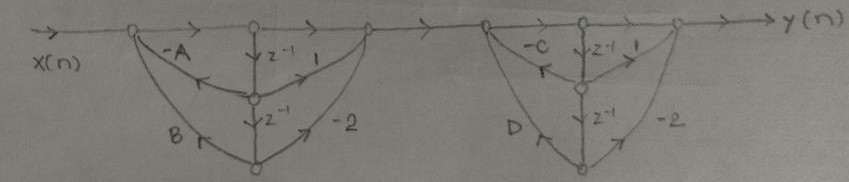
\includegraphics[width=\columnwidth]{figs/lpf-final.jpg}
        \caption{Highpass Digital Filter.}
        \label{fig:lpf-final}
    \end{figure}

    \item We are given the following.
    \begin{align}
        \omega_p = 0.2613\pi,\ \omega_s = 0.4018\pi \\
        20\log_{10}\abs{H_d\brak{e^{j\omega_p}}} \ge -0.75 \text{ dB} \label{eq:mag-pb} \\
        20\log_{10}\abs{H_d\brak{e^{j\omega_s}}} \le -20 \text{ dB} \label{eq:mag-sb}
    \end{align}
    We will use the bilinear transformation method to construct the required
    digital filter from the corresponding analog filter, for which we have
    \begin{align}
        \Omega_p &= \tan\brak{\frac{\omega_p}{2}} = 0.435165 \label{eq:Omega-p} \\
        \Omega_s &= \tan\brak{\frac{\omega_s}{2}} = 0.730871 \label{eq:Omega-s}
    \end{align}
    We also know that the minimum passband magnitude and maximum stopband
    ripple are given by
    \begin{align}
        \abs{H_a\brak{j\Omega_p}}^2 &= \frac{1}{1+\epsilon^2} \label{eq:param-e} \\
        \abs{H_a\brak{j\Omega_s}}^2 &= \frac{1}{A^2} \label{eq:param-A}
    \end{align}
    Since the bilinear transformation does not change magnitude characteristics,
    we substitute \eqref{eq:param-e} in \eqref{eq:mag-pb} and \eqref{eq:param-A}
    in \eqref{eq:mag-sb} to get
    \begin{equation}
        \epsilon^2 = 0.188502,\ A^2 = 100
    \end{equation}
    Hence, the order of the analog Butterworth filter that meets the
    specifications is
    \begin{equation}
        N = \frac{1}{2}\frac{\log_{10}\brak{\frac{A^2-1}{\epsilon^2}}}{\log_{10}\brak{\frac{\Omega_s}{\Omega_p}}} = 6.040140
    \end{equation}
    Taking the ceiling, the order of the analog filter is \(N = 7\). From
    \eqref{eq:param-A},
    \begin{align}
        &\abs{H_a\brak{j\Omega_s}}^2 = \frac{1}{1 + \brak{\frac{\Omega_s}{\Omega_c}}^{2N}} = \frac{1}{A^2} \\
        &\implies \Omega_c = \frac{\Omega_s}{\brak{A^2-1}^{\frac{1}{2N}}} = 0.526375
    \end{align}
    The transfer function of the normalized 7\textsuperscript{th} order
    Butterworth analog filter is
    \begin{equation}
        H_{an}\brak{s} = \prod_{i=1}^7\frac{1}{s-p_i}
        \label{eq:H-an-butter}
    \end{equation}
    where \(p_i,\ 1 \le i \le 7\) are the poles of the normalized Butterworth
    analog filter. De-normalizing \eqref{eq:H-an-butter},
    \begin{equation}
        H_a\brak{s} = H_{an}\brak{\frac{s}{\Omega_c}} = \prod_{i=1}^7\frac{\Omega_c}{s-\Omega_cp_i}
        \label{eq:H-a-butter}
    \end{equation}
    Thus, the poles of the required Butterworth filter are tabulated in
    \autoref{tab:poles-butter}.
    \begin{table}[!ht]
        \centering
        \def\arraystretch{1.05}
        \begin{tabular}{|c|c|}
            \hline
            \(p_i\) & \(p_i' = p_i\Omega_c\) \\
            \hline
            \(-0.9010 + j0.4339\) & \(-0.4743 + j0.2284\) \\
            \hline
            \(-0.9010 - j0.4339\) & \(-0.4743 - j0.2284\) \\
            \hline
            \(-0.6235 + j0.7818\) & \(-0.3283 + j0.4115\) \\
            \hline
            \(-0.6235 - j0.7818\) & \(-0.3283 - j0.4115\) \\
            \hline
            \(-0.2225 + j0.9749\) & \(-0.4743 + j0.2284\) \\
            \hline
            \(-0.2225 - j0.9749\) & \(-0.4743 - j0.2284\) \\
            \hline
            \(-1.000\) & \(-0.5264\) \\
            \hline
        \end{tabular}
        \caption{Poles of the analog Butterworth filter.}
        \label{tab:poles-butter}
    \end{table}
    The transfer function of the corresponding digital filter is obtained as
    \begin{align}
        H_d\brak{z} &= H_a\brak{s}\rvert_{s = \frac{1-z^{-1}}{1+z^{-1}}} \\
        &= \prod_{i=1}^7\frac{\Omega_c\brak{1+z^{-1}}}{\brak{1-p_i'}-\brak{1+p_i'}z^{-1}}
    \end{align}
    where \(p_i'\)'s are as defined in \autoref{tab:poles-butter}.
\end{enumerate}

\end{document}
